\documentclass[a4paper]{article}
\usepackage[german]{babel}
\usepackage{graphicx}
\usepackage{float}

\title{Embedded Systems Praktikum 1}
\author{Finn Bechinka}
\date{26. October 2023}

\begin{document}
\maketitle

\section{Statechart}
\begin{figure}[H]
  \centering
  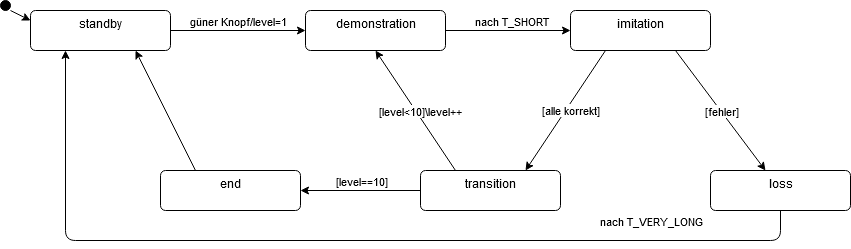
\includegraphics[width=1.0\linewidth]{media/senso-simple.png}
  \caption{State Machine Diagramm (Simpel)}
  \label{fig:statechart-simple}
\end{figure}

\begin{figure}[H]
  \centering
  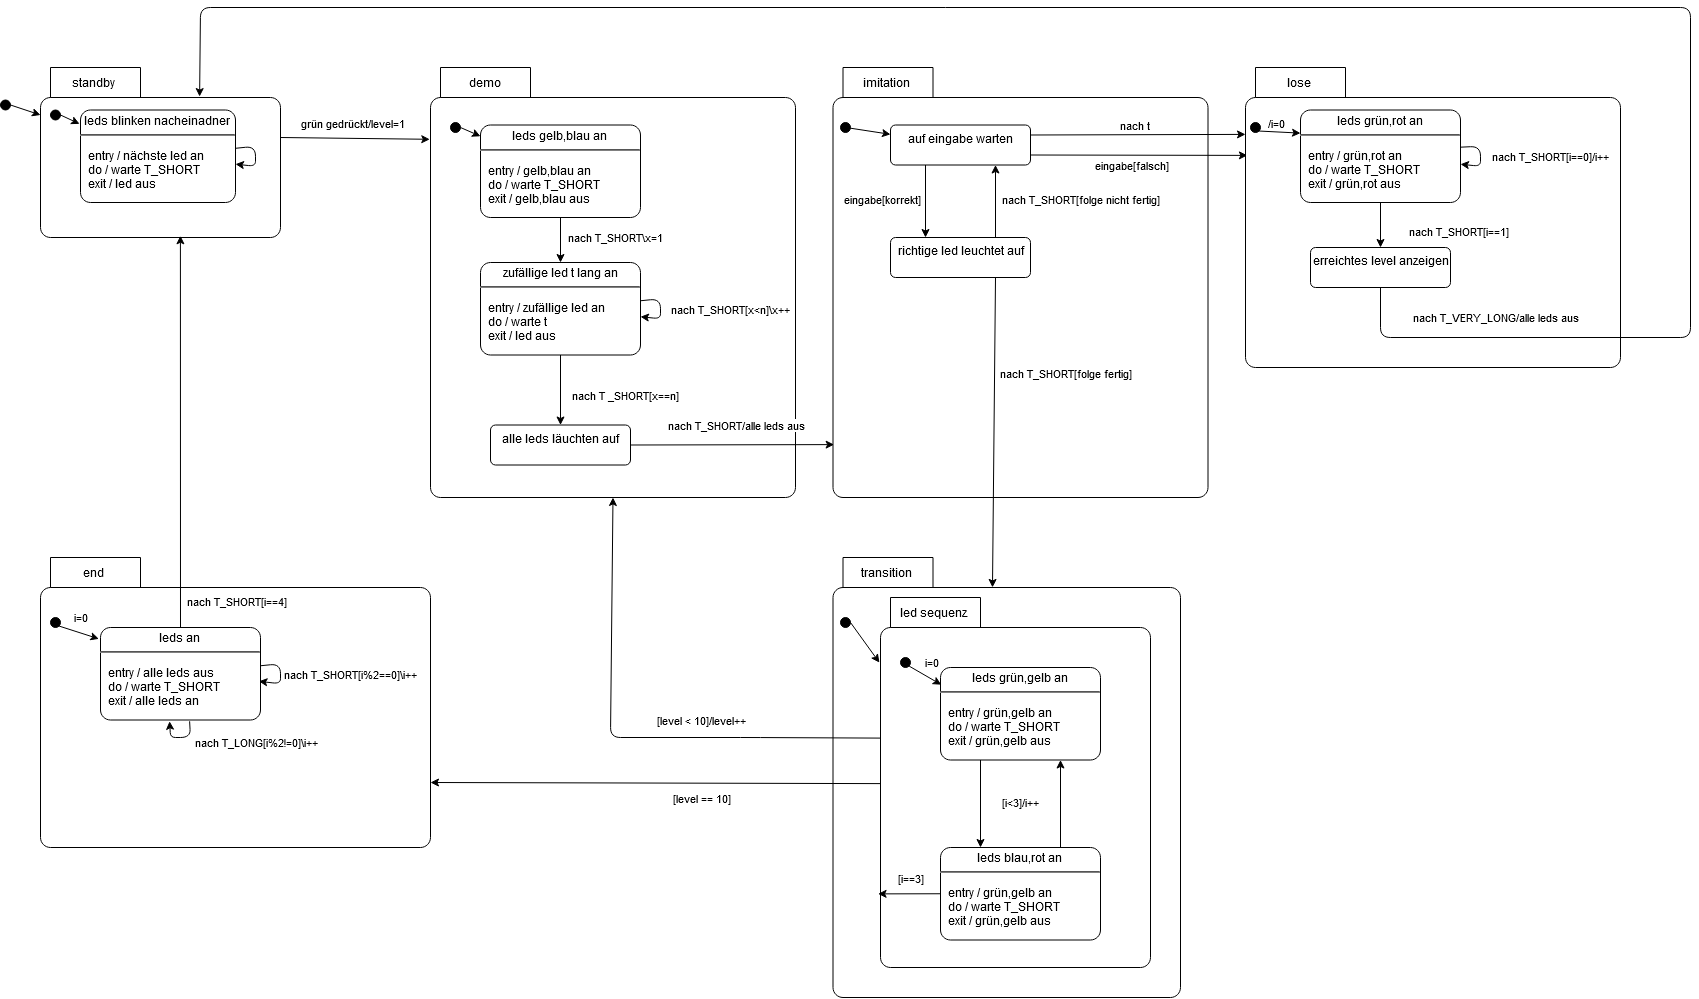
\includegraphics[width=1.0\linewidth]{media/senso-statechart.png}
  \caption{State Machine Diagramm}
  \label{fig:statechat}
\end{figure}

\section{Schaltplan}

\begin{figure}[H]
  \centering
  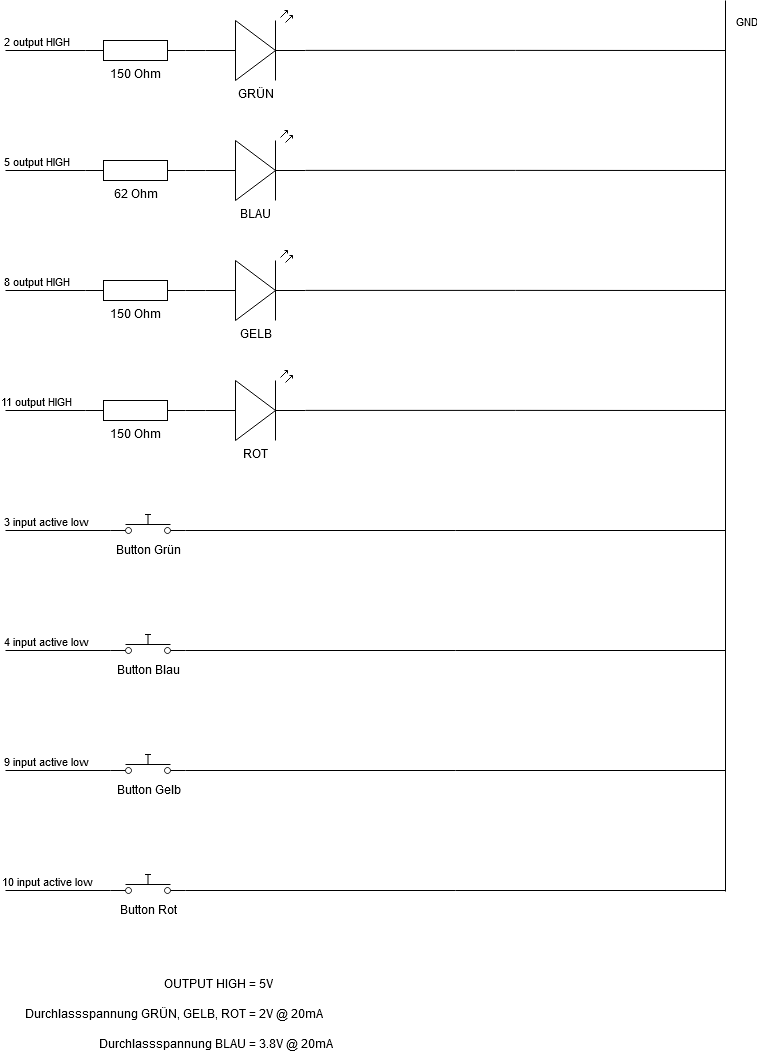
\includegraphics[width=1.0\linewidth]{media/senso-schaltplan.png}
  \caption{Schaltplan}
  \label{fig:schaltplan}
\end{figure}

\end{document}
